\section{No termina de convencerme, pero le voy a dar una oportunidad. ¿Cómo lo instalo?}
  ¡Esa es la actitud!

  Si estas leyendo este libro y eres estudiante, tengo excelentes noticias para ti.
  Si no eres estudiante, tengo no tan excelentes noticias para ti.

  \textit{IntelliJ} viene en dos sabores, sabor \textit{Community} y sabor \textit{Ultimate}.
  Si eres un ser humano común y corriente (o un gato con acceso a internet) puedes descargar e 
  instalar \textit{IntelliJ IDEA Community Edition} desde el sitio oficial de \textit{JetBrains}.
  ¿Muy complicado?
  Totalmente de acuerdo.
  ¿Por qué descargar el \textit{IDE} desde la página web cuando \textit{JetBrains} nos entrega una
  herramienta para facilitarnos el proceso?
  
  %region : JETBRAINS TOOLBOX
  \subsection{JetBrains Toolbox}
    \textit{JetBrains Toolbox}\index{JetBrains Toolbox} es una herramienta que facilita la instalación de los productos de
    \textit{JetBrains}, manejar distintos proyectos y también hace más fácil actualizar las
    herramientas.

    Instalar \textit{Toolbox} se puede hacer descargando la herramienta desde el 
    \href{https://www.jetbrains.com/toolbox-app/}{sitio oficial}.

    Alternativamente, también podemos instalarla desde la terminal.

    \begin{tcolorbox}[enhanced, breakable, title=Windows]
      \begin{powershell}
        winget install JetBrains.Toolbox
      \end{powershell}
    \end{tcolorbox}
    
    \begin{tcolorbox}[enhanced, breakable, title=Linux/Mac]
      \begin{bash}
        BASE_URL="https://data.services.jetbrains.com/products/download"
        PLATFORM="?platform=linux&code=TBA"

        wget --show-progress -qO ./toolbox.tar.gz $BASE_URL$PLATFORM
        
        TOOLBOX_TEMP_DIR=$(mktemp -d)
        tar -C "$TOOLBOX_TEMP_DIR" -xf toolbox.tar.gz
        rm ./toolbox.tar.gz
        "$TOOLBOX_TEMP_DIR"/*/jetbrains-toolbox

        rm -r "$TOOLBOX_TEMP_DIR"
      \end{bash}
    \end{tcolorbox}

    \begin{note}
      \textit{JetBrains} provee de licencias para estudiantes de manera gratuita, para esto, lo único
      que deben hacer es registrarse en  
      \href{https://www.jetbrains.com/es-es/community/education/#students}{el sitio oficial} con su
      correo institucional (por ejemplo, para estudiantes de la Universidad de Chile, puede ser un
      correo \url{@ug.uchile.cl}) y luego solicitar la licencia.
      Con esto podrán acceder a todas las herramientas de \textit{JetBrains} y no tendrán que 
      preocuparse por la licencia.

      Para quienes no son estudiantes, \textit{JetBrains} \textit{IntelliJ IDEA Community Edition} es
      completamente gratis, pero no podrán acceder a todas las herramientas que provee 
      \textit{Ultimate}.
      Lo que suena malo, pero ninguna de las herramientas que no están disponibles en la versión 
      \textit{Community} son necesarias para el desarrollo de este libro. 
      A partir de este momento, cuando se mencione \textit{IntelliJ}, se estará haciendo referencia a
      cualquiera de las dos versiones.
    \end{note}
  %endregion

  \subsection{IntelliJ IDEA}
    \index{IntelliJ IDEA}
    
    En la figura \ref{fig:jb-toolbox} pueden ver la interfaz de \textit{JetBrains Toolbox}, ahí 
    basta con buscar la versión de \textit{IntelliJ} que quieran instalar y hacer click en el botón
    \textit{Install}.

    \begin{figure}[H]
      \centering
      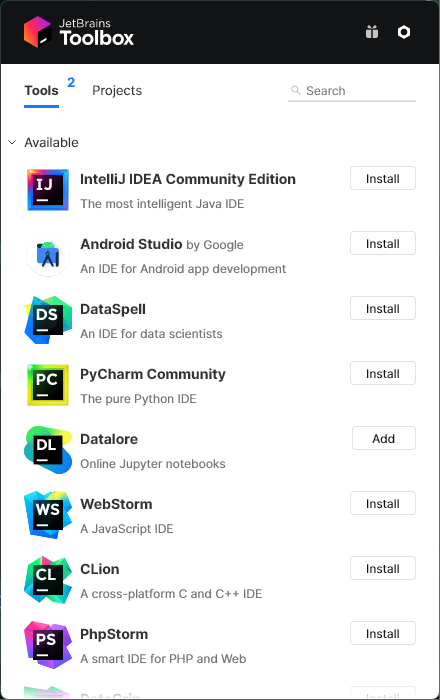
\includegraphics[width=0.4\textwidth]{img/Por_algo_se_empieza/jetbrains-toolbox.png}
      \caption{Interfaz de \textit{JetBrains Toolbox}.}
      \label{fig:jb-toolbox}
    \end{figure}
